\documentclass{article}

\usepackage{fancyhdr} % Required for custom headers
\usepackage{lastpage} % Required to determine the last page for the footer
\usepackage{extramarks} % Required for headers and footers
\usepackage[usenames,dvipsnames]{color} % Required for custom colors
\usepackage{graphicx} % Required to insert images
\usepackage{listings} % Required for insertion of code
\usepackage{courier} % Required for the courier font
\usepackage{lipsum} % Used for inserting dummy 'Lorem ipsum' text into the template
\usepackage{hyperref}
\usepackage{multirow}
\usepackage{tabularx}
\usepackage{framed}
\usepackage{longtable}
\usepackage{listings}
\usepackage{subfigure}
\usepackage{afterpage}
\usepackage{amsmath,amssymb}            
\usepackage{rotating}  
\usepackage{fancyhdr}
\usepackage{graphicx}
\usepackage{amsthm}
\usepackage[scriptsize]{caption} 
\hyphenation{a-gen-tiz-za-zio-ne}
% Margins
\topmargin=-0.45in
\evensidemargin=0in
\oddsidemargin=0in
\textwidth=6.5in
\textheight=9.0in
\headsep=0.25in

\linespread{1.1} % Line spacing

\lstset{
  numbers=left,
  stepnumber=5,    
  firstnumber=1,
  numberfirstline=true
}

% Set up the header and footer
\pagestyle{fancy}
\lhead{\hmwkAuthorName} % Top left header
\chead{\hmwkClass\ (\hmwkClassInstructor\ \hmwkClassTime): \hmwkTitle} % Top center head
\rhead{\firstxmark} % Top right header
\lfoot{\lastxmark} % Bottom left footer
\cfoot{} % Bottom center footer
\rfoot{Page\ \thepage\ of\ \protect\pageref{LastPage}} % Bottom right footer
\renewcommand\headrulewidth{0.4pt} % Size of the header rule
\renewcommand\footrulewidth{0.4pt} % Size of the footer rule

\setlength\parindent{0pt} % Removes all indentation from paragraphs

\usepackage{listings}
\usepackage{color}

\definecolor{dkgreen}{rgb}{0,0.6,0}
\definecolor{gray}{rgb}{0.5,0.5,0.5}
\definecolor{mauve}{rgb}{0.58,0,0.82}

\lstset{frame=tb,
  language=Java,
  aboveskip=3mm,
  belowskip=3mm,
  showstringspaces=false,
  columns=flexible,
  basicstyle={\small\ttfamily},
  numbers=none,
  numberstyle=\tiny\color{gray},
  keywordstyle=\color{blue},
  commentstyle=\color{dkgreen},
  stringstyle=\color{mauve},
  breaklines=true,
  breakatwhitespace=true
  tabsize=3
}

%----------------------------------------------------------------------------------------
%	DOCUMENT STRUCTURE COMMANDS
%	Skip this unless you know what you're doing
%----------------------------------------------------------------------------------------

% Header and footer for when a page split occurs within a problem environment
\newcommand{\enterProblemHeader}[1]{
\nobreak\extramarks{#1}{#1 continued on next page\ldots}\nobreak
\nobreak\extramarks{#1 (continued)}{#1 continued on next page\ldots}\nobreak
}

% Header and footer for when a page split occurs between problem environments
\newcommand{\exitProblemHeader}[1]{
\nobreak\extramarks{#1 (continued)}{#1 continued on next page\ldots}\nobreak
\nobreak\extramarks{#1}{}\nobreak
}




%----------------------------------------------------------------------------------------
%	NAME AND CLASS SECTION
%----------------------------------------------------------------------------------------

\newcommand{\hmwkTitle}{Creational Patterns} % Assignment title
\newcommand{\hmwkDueDate}{Martedi,\ Marzo 31,\ 2015} % Due date
\newcommand{\hmwkClass}{Ingegneria del Software 1} % Course/class
\newcommand{\hmwkClassTime}{} % Class/lecture time
\newcommand{\hmwkClassInstructor}{Claudio Menghi, Alessandro Rizzi} % Teacher/lecturer
\newcommand{\hmwkAuthorName}{} % Your name

%----------------------------------------------------------------------------------------
%	TITLE PAGE
%----------------------------------------------------------------------------------------

\title{
\vspace{2in}
\textmd{\textbf{\hmwkClass:\ \hmwkTitle}}\\
\normalsize\vspace{0.1in}\small{Due\ on\ \hmwkDueDate}\\
\vspace{0.1in}\large{\textit{\hmwkClassInstructor\ \hmwkClassTime}}
\vspace{3in}
}

\author{\textbf{\hmwkAuthorName}}
\date{} % Insert date here if you want it to appear below your name

%----------------------------------------------------------------------------------------

\begin{document}

\maketitle

%----------------------------------------------------------------------------------------
%	TABLE OF CONTENTS
%----------------------------------------------------------------------------------------

%\setcounter{tocdepth}{1} % Uncomment this line if you don't want subsections listed in the ToC

\newpage
\tableofcontents
\newpage



\section{Introduzione}
I problemi incontrati nello sviluppo di grossi progetti software sono spesso ricorrenti e prevedibili
\begin{itemize}
\item I  design pattern sono ``schemi di soluzioni" riutilizzabili
\item  Permettono quindi di non inventare da capo soluzioni ai problemi gi\`a risolti, ma di utilizzare dei ``mattoni" di provata efficacia
\begin{itemize}
\item Un bravo progettista sa riconoscerli, nella documentazione o direttamente nel codice, e utilizzarli per comprendere i programmi scritti da altri
\item forniscono quindi un vocabolario comune che facilita la comunicazione tra progettisti
\end{itemize}
\item Possono rendere la struttura del progetto/codice pi\`u complessa del necessario
\end{itemize}

Un applicazione pu\`o essere suddivisa in tre parti:
\begin{itemize}
\item creazionale: riguarda il processo di creazione degli oggetti
\item strutturale: hanno a che fare con la composizione di classi e oggetti
\item comportamentale: si occupa di come interagiscono gli oggetti
\end{itemize}
Per ognuna di queste parti sono stati identificati dei pattern specifici.  

\subsection{Pattern creazionali}

In questa esercitazione ci focalizziamo sui pattern \texttt{creazionali}. La lista dei pattern creazionali include
\begin{itemize}
\item \emph{Factory method}: viene utilizzato al fine di definire un interfaccia per creare un oggetto, ma lascia alle sottoclassi la decisione del tipo di classe da istanziare;
\item \emph{Abstract Factory}: crea istanze di \emph{famiglie} di oggetti
\item \emph{Singleton}: consente di specificare che \emph{solo} un istanza di una particolare classe esiste.
\item \emph{Prototype}: specifica il tipo di oggetto da creare per mezzo di un istanza prototiplale. Partendo da tale istanza \`e possibile creare nuovi oggetti copiando il prototipo.
\item \emph{Builder}: separa la costruzione di un oggetto complesso dalla sua rappresentazione, in modo che lo stesso processo costruttivo pu\`o portare a differenti rappresentazioni.
\end{itemize}






\subsection{Factory method}
\begin{framed}
\emph{Viene utilizzato al fine di definire un interfaccia per creare un oggetto, ma lascia alle sottoclassi la decisione del tipo di classe da istanziare. Permette alle classi di postporre l'istanziazione di una sottoclasse.}
\end{framed}


Considerate per esempio un framework di applicazioni che devono gestire documenti multipli di un utente. Abbiamo applicazioni diverse, ognuna delle quali fa riferimento a dei documenti di tipo diverso. \`E facile identificare le classi \texttt{Application} e \texttt{Document}, entrambi astratte. Ovviamente lo sviluppatore deve specificare opportune sottoclassi al fine di realizzare implementazioni specifiche delle varie applicazioni. Per esempio, lo sviluppatore potrebbe definire le classi \texttt{DrawingAppliaction} e \texttt{DrawingDocument} che si riferiscono a una specifica applicazione che gestisce documenti ``disegnabili". La classe \texttt{Application} deve essere in grado di creare i vari documenti, per esempio quando l'utente seleziona \texttt{Open}, \texttt{New} da un menu.

Tuttavia, il particolare tipo di documento da istanziare \`e application-specific, la classe \texttt{Application} non conosce \texttt{quando} un documento deve essere creato e \texttt{quale} documento deve essere creato. Il problema \`e che il framework deve istanziare delle classi ma conosce solamente il loro ``tipo astratto" (\texttt{Application} e \texttt{Document}).

Il \texttt{Factory Method} fornisce la soluzione: incapsula la conoscenza relativa al tipo di documento all'interno di una classe esterna. Tale conoscenza viene spostata all'esterno del framework. Il factory method va utilizzato quando 
\begin{itemize}
\item non \`e possibile per una classe anticipare la classe degli oggetti da creare
\item una classe vuole che le sue sottoclassi specifichino il tipo di oggetti da creare
\item la classe delega la responsabilit\`a di creare i sottoelementi alle sue sottoclassi (aiutanti)
\end{itemize}

\begin{figure}[h]
\centering
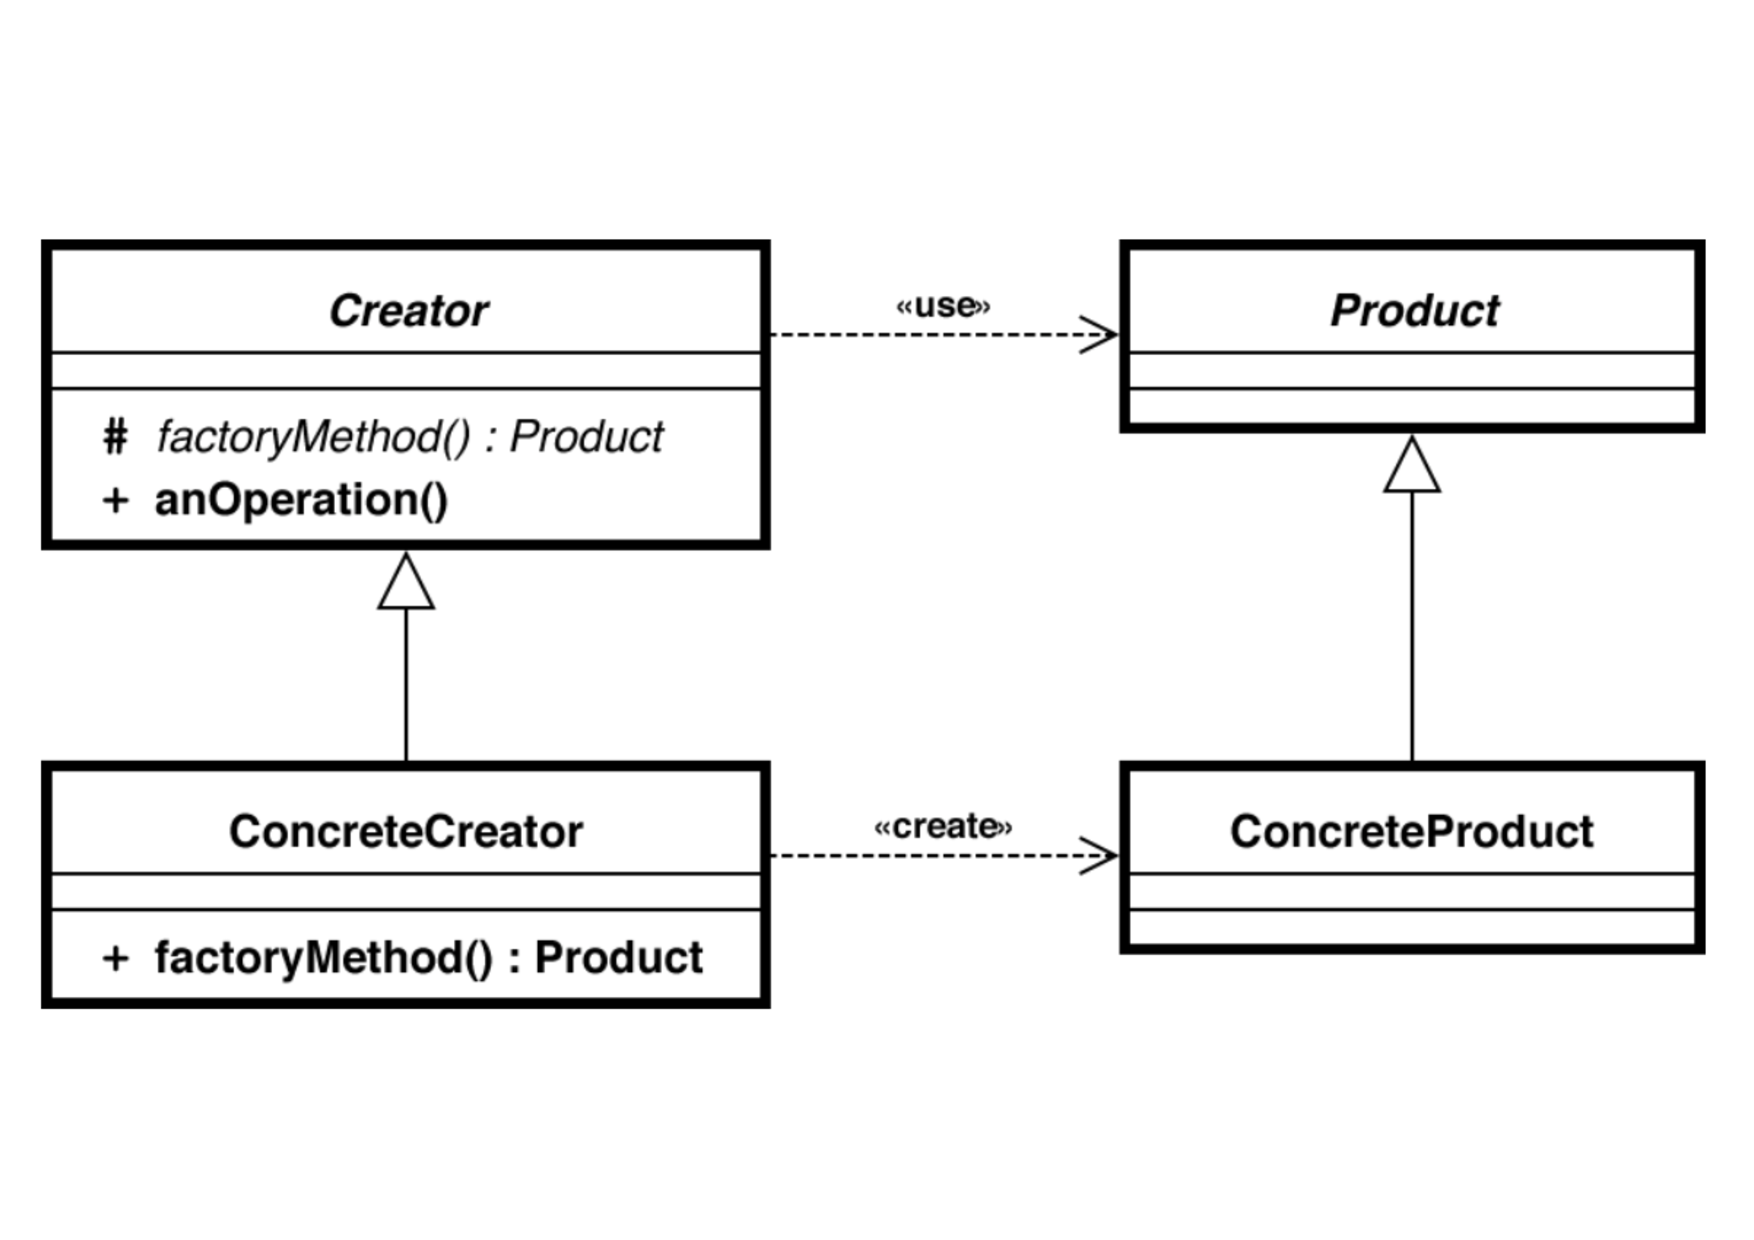
\includegraphics[width=0.5\textwidth]{Img/FactoryMethodDescription.pdf}
\caption{Class diagram relativo al pattern Factory Method}
\label{Fig:FactoryMethodConcepts}
\end{figure}


Il class diagram riferito al factory method \`e descritto in Figura~\ref{Fig:FactoryMethodConcepts}. I componenti principali sono:
\begin{itemize}
\item Product (\texttt{Document}): definisce l'interfaccia o il tipo astratto degli oggetti che il factory method deve creare 
\item ConcreteProduct (\texttt{DrawingDocument}): sono dei prodotti concreti che implementano l'interfaccia o estendono la classe astratta
\item Creator (\texttt{Application}): dichiara il factory method che ritorna un oggetto di tipo Product. Il creatore pu\`o anche definire una implementazione di default che ritorna un oggetto concreto di default
\item ConcreateCreator (\texttt{DrawingAppliaction}): effettua overriding del factory method per fornire un esemplare specifico
\end{itemize}

Ci sono due variazioni del Factory method pattern:
\begin{itemize}
\item il caso in cui il creatore \`e astratto e non fornisce un implementazione per il factory method che dichiara
\item il caso in cui il creatore \`e ``concreto" e fornisce un implementazione di default del factory method.
\end{itemize}

Esistono anche delle versioni parametriche del factory method, che richiedono di passare un parametro al metodo che specifica il tipo di oggetto da creare.

Riguardo agli aspetti implementativi \`e possibile identificare due versioni del factory method:
\begin{itemize}
\item  lazy: crea l'istanza di un oggetto all'interno del \texttt{factoryMethod}. Per esempio, nell'esempio che vedremo in seguito ogni giocattolo viene creato quando viene estratto dal sacco di Babbo Natale.
\item eager: crea l'istanza degli oggetti quando il creatore viene creato. Per esempio, possiamo pensare al creatore come al sacchetto della tombola, nel quale sono inseriti in fase di inizializzazioni i vari numeri che \`e possibile estrarre.
\end{itemize}

Il factory method viene spesso implementato in una versione semplificata mediante un metodo statico all'interno della classe \texttt{Product} stessa o nelle sue sottoclassi. 


\subsection{Abstract factory}
\begin{framed}
Forniscono un interfaccia per creare \emph{famiglie} di prodotti legati tra di loro senza specificare le loro classi concrete.
\end{framed}

Il class diagram replativo al pattern AbstractFactory \`e rappresentato in Figura~\ref{Fig:AbstractFactoryDescription}. L'AbstractFactory pu\`o essere utilizzata per esempio per modellizzare applicazioni con multipli \emph{look-and-feel} standards. Diversi \emph{look-and-feel} aggregano componenti diverse: diverse scrool bars, finestre e bottoni. Per esempio, se l'applicazione viene eseguita su un pc, determinate scrool bars (\texttt{ProductA1}), finestre (\texttt{ProductB1}) e bottoni vengono selezionate mentre se viene eseguito su un tablet un altro insieme di scrool bars (\texttt{ProductA2}), finestre (\texttt{ProductB2}) e bottoni viene selezionato. La soluzione consiste nello specificare per ogni componente i relativi sottocomponenti corrispondenti ai diversi \emph{look-and-feel}. Per ogni \emph{look-and-feel} pc e tablet ci sar\`a una appropriata factory (\texttt{ConcreteFactory1} e \texttt{ConcreteFactory2}) che aggrega i componenti corrispondenti alla specifica istanza di prodotto che si vuole ottenere.

\begin{figure}[h]
\centering
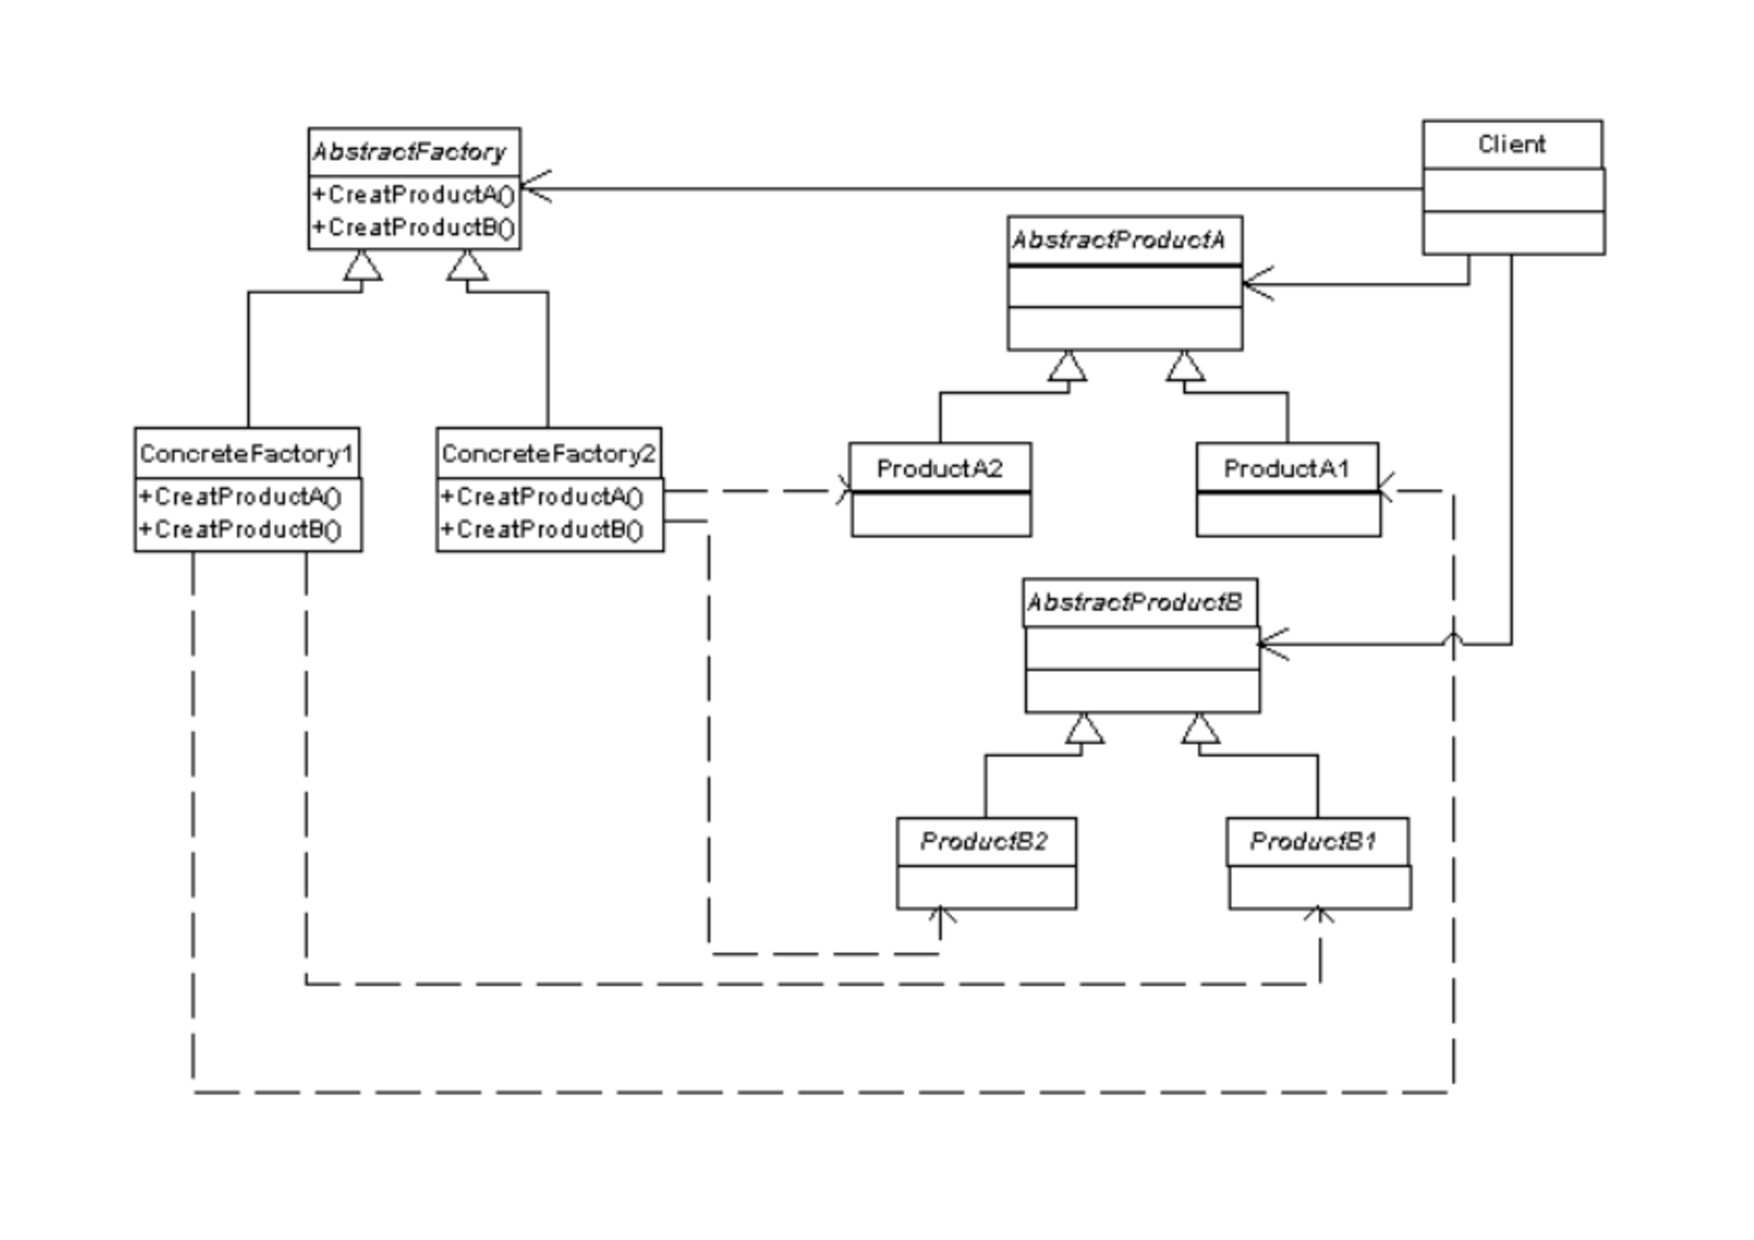
\includegraphics[width=1\textwidth]{Img/AbstractFactoryDescription.pdf}
\caption{Class diagram relativo al pattern AbstractFactory}
\label{Fig:AbstractFactoryDescription}
\end{figure}

I componenti dell'AbstractFactory sono:
\begin{itemize}
\item AbstractFactory: dichiara un interfaccia che contiene le operazioni per creare i prodotti
\item ConcreteFactory: implementa le operazioni per creare i vari oggetti
\item AbstractProduct: definisce le interfacce dei veri prodotti
\item ConcreteProduct: definisce un oggetto ``concreto" che pu\`o essere utilizzato dalle factories
\end{itemize}

In genere una sola istanza delle concrete factories viene creata a run-time. Le factory concrete possono essere implementate utilizzando il Prototype pattern.





\subsection{Singleton}
\begin{framed}
\emph{Viene utilizzato al fine di garantire che esiste \textbf{una sola} istanza di una specifica classe, e fornisce un punto di accesso ad essa.}
\end{framed}

Ci sono classi che devono avere una sola istanza all'interno del sistema, per esempio sebbene ci possano essere pi\`u stampanti deve esistere uno solo spooler di stampa.
Per garantire che ci sia una sola istanza di una classe \texttt{A} potremmo dichiarare un unica variabile, ma ci\`o non ci vieta di dichiarare questa variabile pi\`u volte o in altre parti del codice.
Al fine di avere la garanzia che solo un istanza della classe \texttt{A} esista \`e necessario rendere la classe \texttt{A}  stessa  responsabile della sua creazione e di ``tenere" traccia della sua unica istanza. La classe deve garantire che non \`e possibile creare altre istanze della classe \texttt{A} e deve fornire un metodo che garantisce l'accesso alla sua unica istanza.

\begin{figure}[h]
\centering
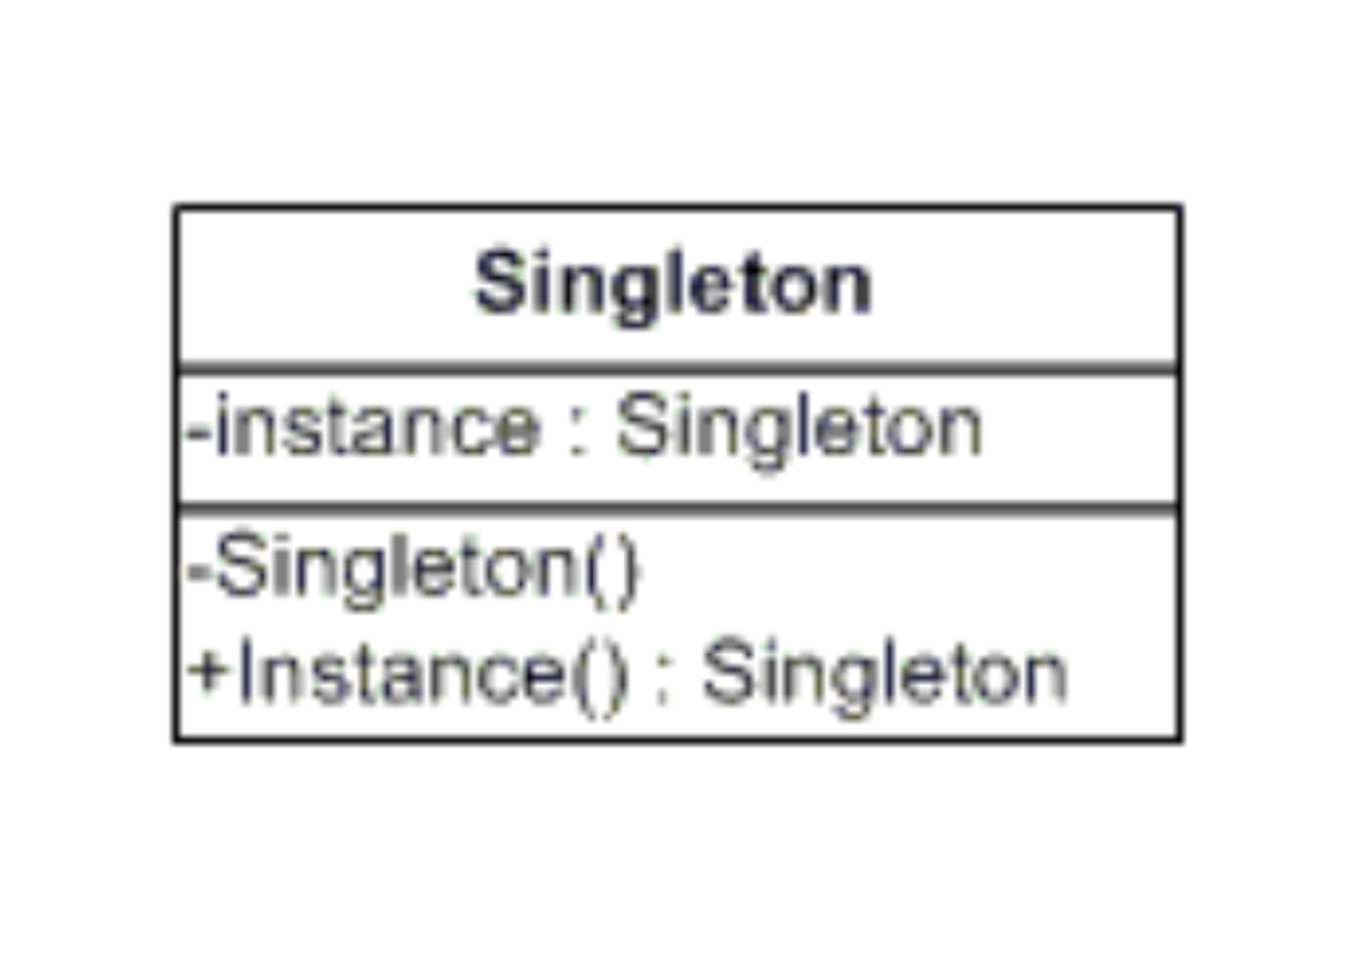
\includegraphics[width=0.3\textwidth]{Img/Singleton.pdf}
\caption{Diagramma UML relativo al Singleton Pattern}
\label{Fig:Singleton}
\end{figure}

Il singleton pattern descritto in Figura~\ref{Fig:Singleton} richiede di dichiarare un attributo statico \texttt{instance} che contiene l'unico oggetto della classe \texttt{Singleton} considerata. Il costruttore della classe viene reso privato e reso accessibile mediante il metodo statico \texttt{getInstance} (in Figura il metodo viene indicato con il nome \texttt{Instance}).
Il singleton pattern ha le seguenti caratteristiche:
\begin{itemize}
\item \emph{accesso controllato all'unica istanza}: visto che la classe Singleton encapsula l'unica \emph{istanza} della classe ha il controllo di come e quando i client possono accedere all'istanza condivisa.
\item \emph{pu\`o essere estesa} la classe pu\`o essere estesa ed \`e semplice riconfigurare l'applicazione per ritornare un istanza della classe estesa. 
\item \emph{fornisce un numero variabile di istanze}: il pattern consente di gestire pi\`u di una istanza all'interno della Singleton class. 
\end{itemize}
Nota che il costruttore \`e \texttt{private} (in particolari casi potrebbe anche essere dichiarato \texttt{protected}). Un client che prova a inizializzare un \texttt{Singleton} utilizzando il costruttore avr\`a un errore a compile time: non pu\`o accedere al costruttore visto che \`e privato. Questo garantisce che una sola istanza potr\`a essere creata, e sar\`a accessibile mediante il metodo \texttt{getInstance}. A seconda di quando viene creata l'unica istanza possiamo avere diverse implementazioni del patter \texttt{Singleton}.

\subsubsection{Lazy singleton}
Il lazy singleton \`e una specifica implementazione del Singleton pattern che non crea l'istanza finch\`e il metodo \texttt{getInstance} non viene invocato per la prima volta.
\begin{lstlisting}[language=Java]
public class Singleton {
	// istanza singola
	private static Singleton instance;

	// costruttore
	private Singleton() {
	}

	public static Singleton getInstance() {
		// crea l’oggetto solo se non esiste
		if (instance == null) {
			instance = new Singleton();
		}
		return instance;
	}
	// altri metodi
}
\end{lstlisting}
Nota che questa implementazione \`e scorreta in ambito multithreading: in tal caso \`e possibile che il metodo \texttt{getInstance} ritorni due  istanze diverse della classe \texttt{Singleton}.

\subsubsection{Eager Singleton}
L'eager singleton \`e una specifica implementazione del Singleton pattern che crea l'istanza in fase di inizializzazione. 
\begin{lstlisting}[language=Java]
public class Singleton {
	// istanza singola
	private static Singleton instance=new Singleton();

	// costruttore
	private Singleton() {
	   
	}

	public static Singleton getInstance() {
		return instance;
	}
	// altri metodi
}
\end{lstlisting}
Nota che questa implementazione \`e correta in ambito multithreading.

\subsubsection{Enum Singleton}
Questo approccio sfrutta il fatto che un valore di enum viene istanziato una volta sola in un programma Java. 
\begin{lstlisting}[language=Java]
public enum Singleton {
	INSTANCE;
	
	private final int num;
	
	private Singleton(){
		this.num=0;
	}
	
	public static Singleton getInstance(){
		return INSTANCE;
	}

	public int getNum() {
		return num;
	}
}
\end{lstlisting}
Nota che questa implementazione \`e correta in ambito multithreading. Lo svantaggio \`e che l'implementazione non \`e flessibile: non posso fare sub-classing.

\subsubsection{Synchronized Lazy Singleton}
\`E una versione del  Lazy Singleton corretta in ambito multithreading. Lo svantaggio \`e che i metodi synchronized in generale possono essere inefficienti.
\begin{lstlisting}[language=Java]
public class Singleton {
	private static Singleton uniqueInstance;
	
	private Singleton(){
		// costruttore
	}
	
	// metodi synchronized possono essere inefficienti
	public static synchronized Singleton getInstance(){
		if (uniqueInstance == null){
			uniqueInstance = new Singleton();
		}
		return uniqueInstance;
	}
}
\end{lstlisting}

\clearpage
\section{Esercizi}



\subsection{Esercizio 1: Factory method}
\begin{framed}
Esercizio 1: implementare un gioco contenente un labirinto. Il labirinto deve essere composto da locali, porte e muri. Ogni locale ha quattro pareti, nord sud est ovest che possono essere occupati da un muro o da una porta. Deve essere possibile anche creare un tipo di labirinto bombato (esplosivo), dove ogni 3 porte viene creata una porta bombata (esplosiva).
\end{framed}


\begin{figure}[h]
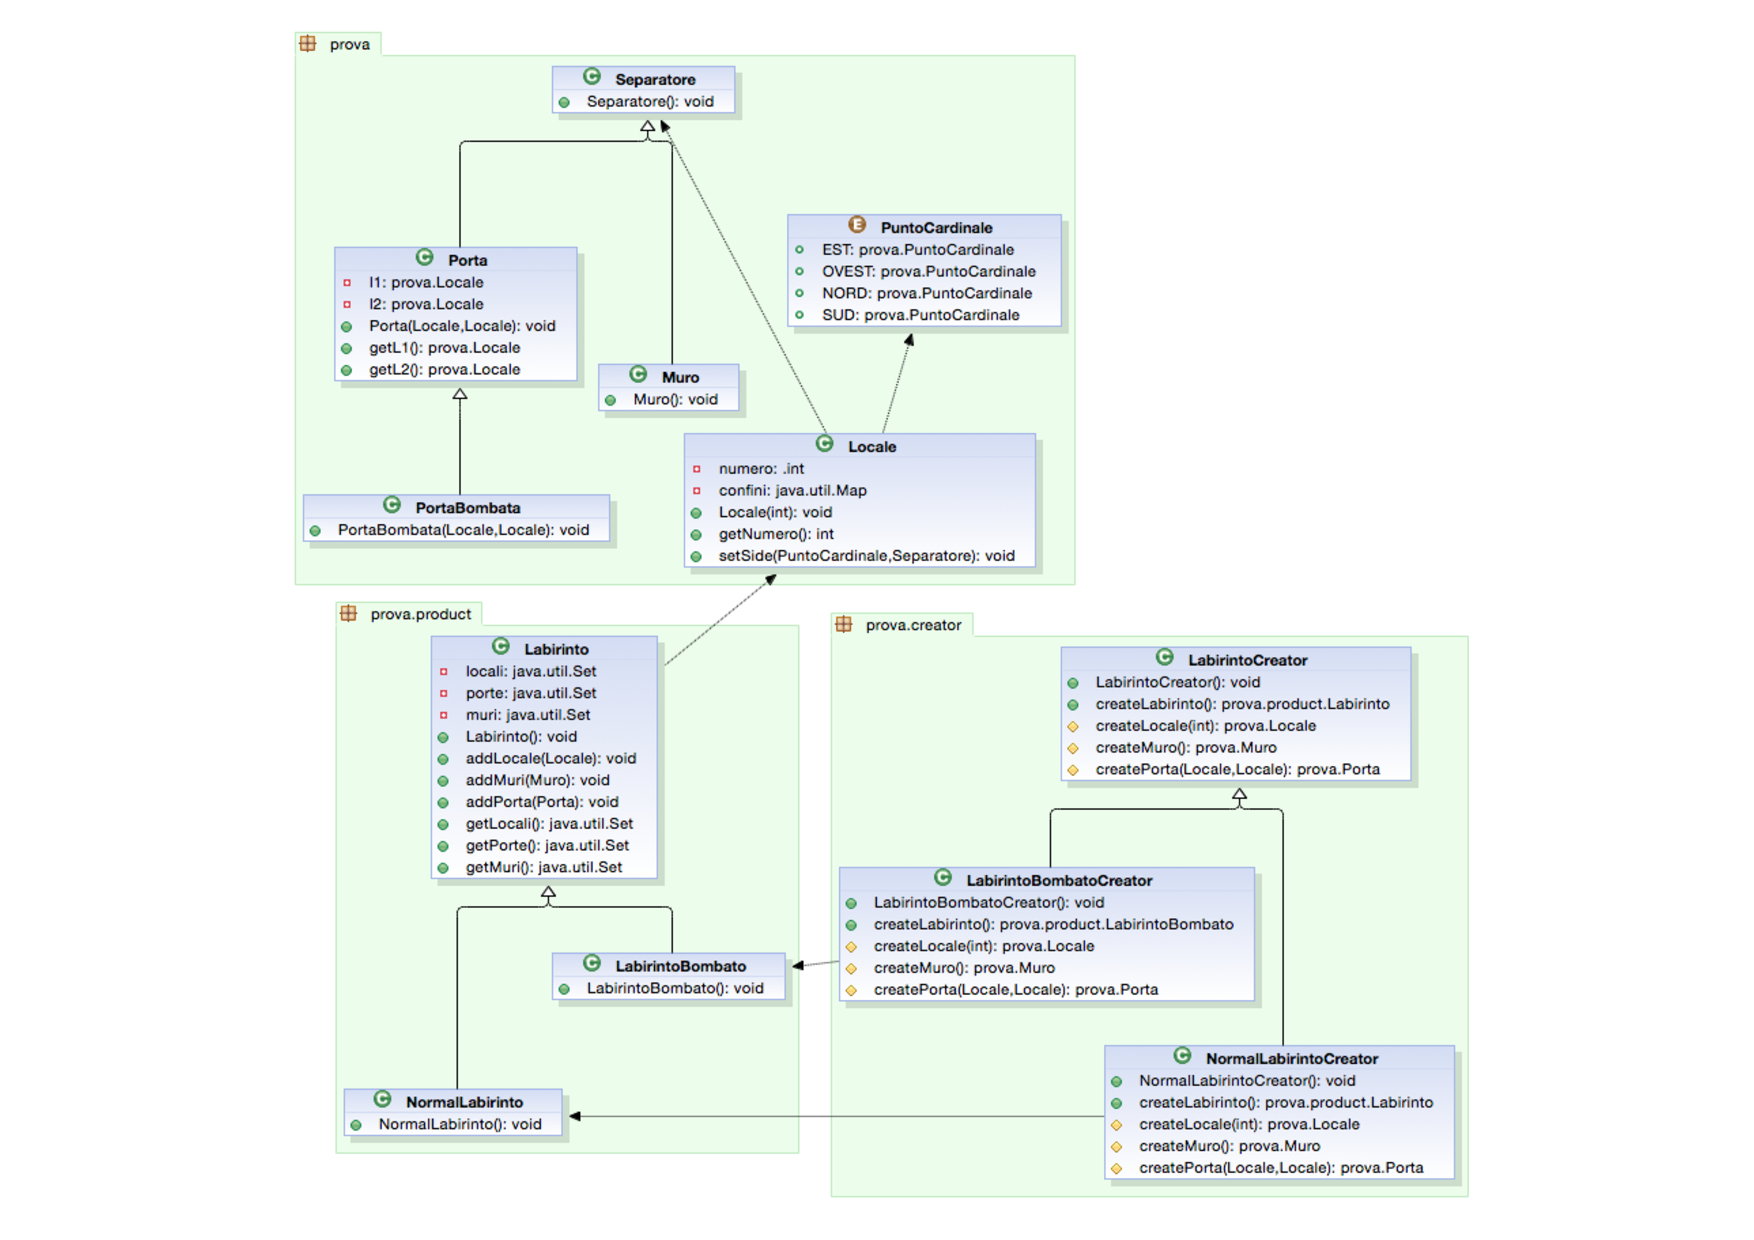
\includegraphics[width=1\textwidth]{Img/FactoryMethod.pdf}
\caption{Class Diagram relativo alla soluzione dell'esercizio 1}
\label{Fig:labirinto}
\end{figure}

Iniziamo modellizzando il labirinto~\ref{Fig:labirinto} mediante la classe \texttt{Labirinto}. Il labirinto \`e composto da vari \texttt{Locali}. Ogni locale \`e identificato per mezzo di un intero. Il locale ha quattro confini: \texttt{NORD},\texttt{SUD}, \texttt{EST} e \texttt{OVEST}, rappresentati per mezzo di un \texttt{enum}. In ognuno di questi confini \`e posto un \texttt{Separatore}. Il separatore pu\`o essere una \texttt{Porta} o un \texttt{Muro}. Una porta memorizza i due locali che connette. Una \texttt{PortaBombata} \`e un particolare tipo di porta che espode una volta aperta. 

Un \texttt{Labirinto} pu\`o essere di due tipi \texttt{NormalLabirinto} e \texttt{LabirintoBombato}. Un \texttt{NormalLabirinto} contiene solo porte normali mentre un \texttt{LabirintoBombato} ogni 3 porte ne contiene una bombata. 

Per creare i due tipi di labirinto decidiamo di utilizzare il pattern \texttt{FactoryMethod}. Dichiariamo un creator astratto \texttt{LabirintoCreator} da cui ereditano i due creator ``concreti" \texttt{LabirintoBombatoCreator} e \texttt{NormalLabirintoCreator}. Questa soluzione ci permette di essere molto flessibili. Per esempio il nostro \texttt{Gioco} potrebbe ``ragionare" in termini di \texttt{Labirinto} astratti. In fase di inizializzazione passiamo come parametro il creator desiderato: se desideriamo creare un gioco che lavora su un labirinto bombato passiamo una istanza di \texttt{LabirintoBombatoCreator}, mentre se desideriamo giocare su un labirinto normale passiamo un istanza di \texttt{NormalLabirintoCreator}.
A seconda del creatore passato in fase di inizializzazione possiamo ottenere giochi dal comportamento totalmente diverso. Per esempio, nel caso di un \texttt{LabirintoBombato} un giocatore potrebbe morire dopo aver aperto una \texttt{PortaBombata}.



\subsubsection{Locale}
\begin{lstlisting}[language=Java]
public class Locale {
	
	private final int numero;
	private final Map<PuntoCardinale, Separatore> confini;
	
	public Locale(int numero){
		this.numero=numero;
		this.confini=new HashMap<PuntoCardinale, Separatore>();
	}

	public int getNumero() {
		return numero;
	}
	
	public void setSide(PuntoCardinale p, Separatore s){
		this.confini.put(p, s);
	}

	@Override
	public int hashCode() {
		final int prime = 31;
		int result = 1;
		result = prime * result + ((confini == null) ? 0 : confini.hashCode());
		result = prime * result + numero;
		return result;
	}

	@Override
	public boolean equals(Object obj) {
		if (this == obj)
			return true;
		if (obj == null)
			return false;
		if (getClass() != obj.getClass())
			return false;
		Locale other = (Locale) obj;
		if (confini == null) {
			if (other.confini != null)
				return false;
		} else if (!confini.equals(other.confini))
			return false;
		if (numero != other.numero)
			return false;
		return true;
	}
}
\end{lstlisting}

\subsubsection{Muro}
\begin{lstlisting}[language=Java]
public class Muro extends Separatore{

	public Muro() {
		super();
	}
}
\end{lstlisting}

\subsubsection{Porta}
\begin{lstlisting}[language=Java]
public class Porta extends Separatore{

	private final Locale l1;
	private final Locale l2;
	
	public Porta(Locale l1, Locale l2){
		super();
		this.l1=l1;
		this.l2=l2;
	}

	public Locale getL1() {
		return l1;
	}

	public Locale getL2() {
		return l2;
	}
	
	public void apri(){
		System.out.println("E' possibile muoversi da "+l1+" a l2"+l2);
	}

	@Override
	public int hashCode() {
		final int prime = 31;
		int result = 1;
		result = prime * result + ((l1 == null) ? 0 : l1.hashCode());
		result = prime * result + ((l2 == null) ? 0 : l2.hashCode());
		return result;
	}

	@Override
	public boolean equals(Object obj) {
		if (this == obj)
			return true;
		if (obj == null)
			return false;
		if (getClass() != obj.getClass())
			return false;
		Porta other = (Porta) obj;
		if (l1 == null) {
			if (other.l1 != null)
				return false;
		} else if (!l1.equals(other.l1))
			return false;
		if (l2 == null) {
			if (other.l2 != null)
				return false;
		} else if (!l2.equals(other.l2))
			return false;
		return true;
	}
}
\end{lstlisting}

\subsubsection{PortaBombata}
\begin{lstlisting}[language=Java]
public class PortaBombata extends Porta {

	public PortaBombata(Locale l1, Locale l2) {
		super(l1, l2);
	}

	public void apri(){
		System.out.println("Bum");
	}
}
\end{lstlisting}


\subsubsection{PuntoCardinale}
\begin{lstlisting}[language=Java]
public enum PuntoCardinale {
	NORD, SUD, EST, OVEST;
}
\end{lstlisting}

\subsubsection{Separatore}
\begin{lstlisting}[language=Java]
public abstract class Separatore {	
}
\end{lstlisting}


\subsubsection{Labirinto}
\begin{lstlisting}[language=Java]
public abstract class Labirinto {

	private final Set<Locale> locali;
	
	public Labirinto(){
		this.locali=new HashSet<Locale>();
	}

	
	public void addLocale(Locale l){
		this.locali.add(l);
	}

	public Set<Locale> getLocali() {
		return locali;
	}
}
\end{lstlisting}

\subsubsection{LabirintoBombato}
\begin{lstlisting}[language=Java]
public class LabirintoBombato extends Labirinto {

}
\end{lstlisting}

\subsubsection{NormalLabirinto}
\begin{lstlisting}[language=Java]
public class NormalLabirinto extends Labirinto{
	
}
\end{lstlisting}

\subsubsection{LabirintoCreator}
\begin{lstlisting}[language=Java]
public abstract class LabirintoCreator {
	
	public abstract Labirinto createLabirinto();

	protected abstract Muro createMuro();
	
	protected abstract Locale createLocale(int numero);
	
	protected abstract Porta createPorta(Locale l1, Locale l2);
	
}
\end{lstlisting}

\subsubsection{LabirintoBombatoCreator}
\begin{lstlisting}[language=Java]
public class LabirintoBombatoCreator extends LabirintoCreator {
	
	private int counter=0;
	public LabirintoBombato createLabirinto(){
		
		LabirintoBombato labirinto=new LabirintoBombato();
		Locale l1=this.createLocale(1);
		Locale l2=this.createLocale(2);
		
		Porta p1=this.createPorta(l1, l2);
		
		labirinto.addLocale(l1);
		labirinto.addLocale(l2);
		
		l1.setSide(PuntoCardinale.NORD, this.createMuro());
		l1.setSide(PuntoCardinale.EST, p1);
		l1.setSide(PuntoCardinale.SUD, this.createMuro());
		l1.setSide(PuntoCardinale.OVEST, this.createMuro());
		
		l2.setSide(PuntoCardinale.NORD, this.createMuro());
		l2.setSide(PuntoCardinale.EST, this.createMuro());
		l2.setSide(PuntoCardinale.SUD, this.createMuro());
		l2.setSide(PuntoCardinale.OVEST, p1);
		
		return labirinto;
	}
	
	protected Muro createMuro(){
		return new Muro();
	}
	
	protected Locale createLocale(int numero){
		return new Locale(numero);
		
	}
	
	protected Porta createPorta(Locale l1, Locale l2){
		if(counter%3==0){
			return new PortaBombata(l1, l2);
		}
		else{
			return new Porta(l1, l2);
		}
	}
}
\end{lstlisting}

\subsubsection{NormalLabirintoCreator}

\begin{lstlisting}[language=Java]
public class NormalLabirintoCreator extends LabirintoCreator{
	
	
	public NormalLabirinto createLabirinto(){
		NormalLabirinto labirinto=new NormalLabirinto();
		Locale l1=this.createLocale(1);
		Locale l2=this.createLocale(2);
		
		Porta p1=this.createPorta(l1, l2);
		
		labirinto.addLocale(l1);
		labirinto.addLocale(l2);
		
		l1.setSide(PuntoCardinale.NORD, this.createMuro());
		l1.setSide(PuntoCardinale.EST, p1);
		l1.setSide(PuntoCardinale.SUD, this.createMuro());
		l1.setSide(PuntoCardinale.OVEST, this.createMuro());
		
		l2.setSide(PuntoCardinale.NORD, this.createMuro());
		l2.setSide(PuntoCardinale.EST, this.createMuro());
		l2.setSide(PuntoCardinale.SUD, this.createMuro());
		l2.setSide(PuntoCardinale.OVEST, p1);
		
		return labirinto;
	}
	
	protected Muro createMuro(){
		return new Muro();
	}
	
	protected Locale createLocale(int numero){
		return new Locale(numero);
		
	}
	
	protected Porta createPorta(Locale l1, Locale l2){
		return new Porta(l1, l2);
	}
	
}
\end{lstlisting}

\subsection{Esercizio 2: Abstract Factory}
\begin{framed}
Esercizio 2: Deve essere possibile creare labirinti di vario tipo. Per esempio un labirinto incantato deve contenere dei locali incantati, delle porte parlanti etc. Un labirinto esterno contiene delle porte in sasso (per aprire tale porte \`e necessario avere una determinata energia), i muri sono siepi etc.
\end{framed}
In questo caso abbiamo a che fare con delle \emph{famiglie} di prodotti legati tra di loro. Abbiamo un insieme di classi astratte \texttt{Labirinto}, \texttt{Locale}, \texttt{Muro} e \texttt{Porta}. Abbiamo due tipi di labirinti: \texttt{LabirintoMagico} e \texttt{LabirintoEsterno}. Ognuno degli elementi visti in precedenza (\texttt{Locale}, \texttt{Muro} e \texttt{Porta}) ha una specializzazione relativa al \texttt{LabirintoMagico} e una relativa al \texttt{LabirintoEsterno}: \texttt{LocaleMagico}, \texttt{MuroMagico} e \texttt{PortaMagica} si riferiscono al \texttt{LabirintoMagico} mentre \texttt{Giardino}, \texttt{Siepe} e \texttt{Sasso} si riferiscono a \texttt{LabirintoEsterno}. \`E evidente che il pattern creazionale pi\`u adatto al metodo in questione \`e l'Abstract Factory, il quale consente di specificare un interfaccia (o classe astratta) \texttt{LabirintoCreator} che consente di creare  \texttt{famiglie} di oggetti dipendenti senza specificare le loro classi concreto. Le sottoclassi \texttt{LabirintoEsternoCreator} e \texttt{LabirintoMagicoCreator} contengono la logica di creazionale di un  \texttt{LabirintoMagico} e di un \texttt{LabirintoEsterno}.
\begin{figure}
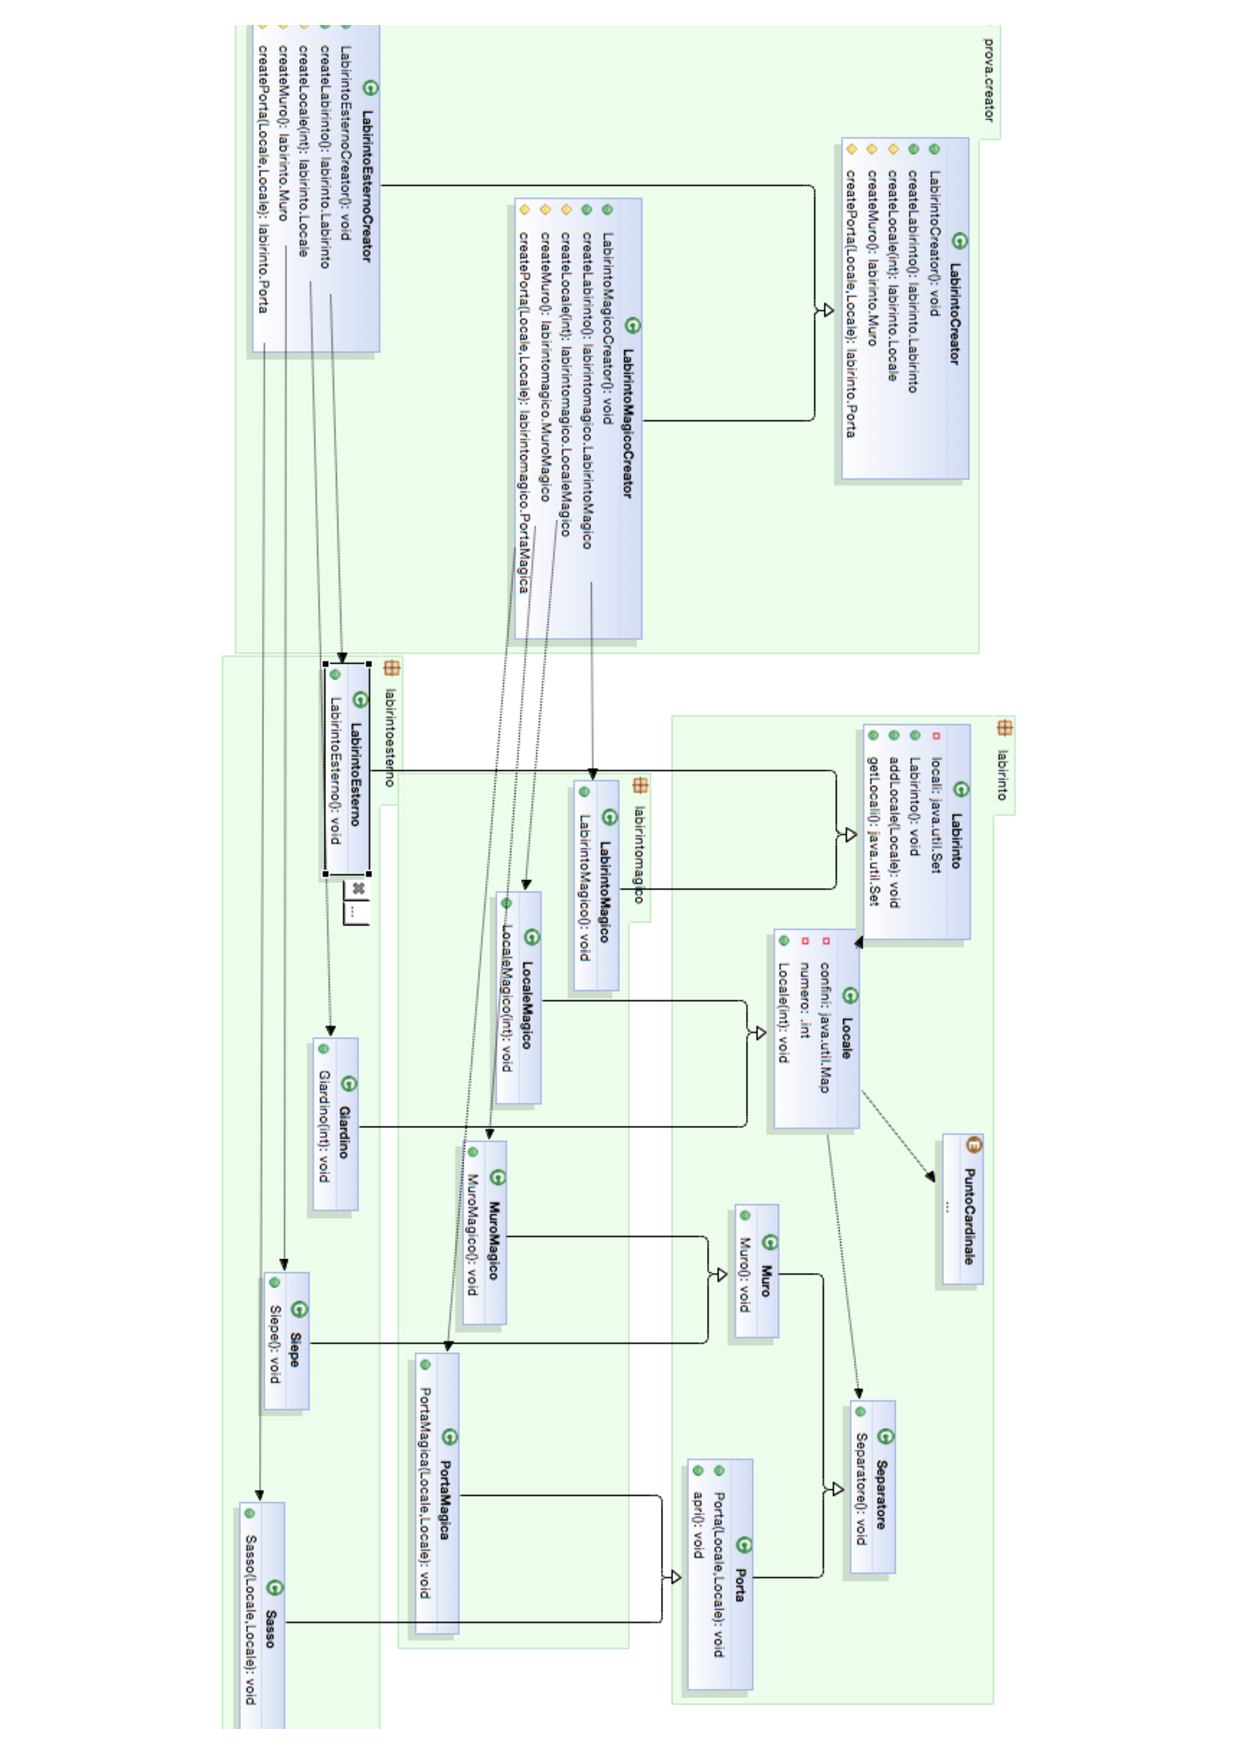
\includegraphics[width=0.8\textwidth]{Img/AbstractFactoryLabirinti2.pdf}
\caption{Class Diagram relativo alla soluzione dell'esercizio 2}
\label{Fig:labirintoMagico}
\end{figure}

\subsubsection{Labirinto}
\begin{lstlisting}[language=Java]
public abstract class Labirinto {

	private final Set<Locale> locali;
	
	public Labirinto(){
		this.locali=new HashSet<Locale>();
	}

	
	public void addLocale(Locale l){
		this.locali.add(l);
	}

	public Set<Locale> getLocali() {
		return locali;
	}
}
\end{lstlisting}

\subsubsection{Locale}
\begin{lstlisting}[language=Java]
public abstract class Locale {
	
	private final int numero;
	private final Map<PuntoCardinale, Separatore> confini;
	
	public Locale(int numero){
		this.numero=numero;
		this.confini=new HashMap<PuntoCardinale, Separatore>();
	}

	public int getNumero() {
		return numero;
	}
	
	public void setSide(PuntoCardinale p, Separatore s){
		this.confini.put(p, s);
	}

	@Override
	public int hashCode() {
		final int prime = 31;
		int result = 1;
		result = prime * result + ((confini == null) ? 0 : confini.hashCode());
		result = prime * result + numero;
		return result;
	}

	@Override
	public boolean equals(Object obj) {
		if (this == obj)
			return true;
		if (obj == null)
			return false;
		if (getClass() != obj.getClass())
			return false;
		Locale other = (Locale) obj;
		if (confini == null) {
			if (other.confini != null)
				return false;
		} else if (!confini.equals(other.confini))
			return false;
		if (numero != other.numero)
			return false;
		return true;
	}
}
\end{lstlisting}

\subsubsection{Muro}
\begin{lstlisting}[language=Java]
public abstract class Muro extends Separatore{

	public Muro() {
		super();
	}
}
\end{lstlisting}

\subsubsection{Porta}
\begin{lstlisting}[language=Java]
public abstract class Porta extends Separatore{

	private final Locale l1;
	private final Locale l2;
	
	public Porta(Locale l1, Locale l2){
		super();
		this.l1=l1;
		this.l2=l2;
	}

	public Locale getL1() {
		return l1;
	}

	public Locale getL2() {
		return l2;
	}
	
	public void apri(){
		System.out.println("E' possibile muoversi da "+l1+" a l2"+l2);
	}

	@Override
	public int hashCode() {
		final int prime = 31;
		int result = 1;
		result = prime * result + ((l1 == null) ? 0 : l1.hashCode());
		result = prime * result + ((l2 == null) ? 0 : l2.hashCode());
		return result;
	}

	@Override
	public boolean equals(Object obj) {
		if (this == obj)
			return true;
		if (obj == null)
			return false;
		if (getClass() != obj.getClass())
			return false;
		Porta other = (Porta) obj;
		if (l1 == null) {
			if (other.l1 != null)
				return false;
		} else if (!l1.equals(other.l1))
			return false;
		if (l2 == null) {
			if (other.l2 != null)
				return false;
		} else if (!l2.equals(other.l2))
			return false;
		return true;
	}
}
\end{lstlisting}

\subsubsection{PuntoCardinale}
\begin{lstlisting}[language=Java]
public enum PuntoCardinale {
	NORD, SUD, EST, OVEST;
}
\end{lstlisting}

\subsubsection{Separatore}
\begin{lstlisting}[language=Java]
public abstract class Separatore {
	
}
\end{lstlisting}

\subsubsection{Giardino}
\begin{lstlisting}[language=Java]
public class Giardino extends Locale {

	public Giardino(int numero) {
		super(numero);
	}
}
\end{lstlisting}

\subsubsection{Labirinto Esterno}
\begin{lstlisting}[language=Java]
public class LabirintoEsterno extends Labirinto {

}
\end{lstlisting}

\subsubsection{Sasso}
\begin{lstlisting}[language=Java]
public class Sasso extends Porta {

	public Sasso(Locale l1, Locale l2) {
		super(l1, l2);
	}
}
\end{lstlisting}

\subsubsection{Siepe}
\begin{lstlisting}[language=Java]
public class Siepe extends Muro {

}
\end{lstlisting}

\subsubsection{Labirinto Magico}
\begin{lstlisting}[language=Java]
public class LabirintoMagico extends Labirinto {

}
\end{lstlisting}

\subsubsection{Locale Magico}
\begin{lstlisting}[language=Java]
public class LocaleMagico extends Locale {

	public LocaleMagico(int numero) {
		super(numero);
	}
}
\end{lstlisting}

\subsubsection{Muro Magico}
\begin{lstlisting}[language=Java]
public class MuroMagico extends Muro {

}
\end{lstlisting}

\subsubsection{PortaMagica}
\begin{lstlisting}[language=Java]
public class PortaMagica extends Porta {

	public PortaMagica(Locale l1, Locale l2) {
		super(l1, l2);
	}
}
\end{lstlisting}
\subsubsection{LabirintoCreator}
\begin{lstlisting}[language=Java]
public abstract class LabirintoCreator {
	
	public abstract Labirinto createLabirinto();

	protected abstract Muro createMuro();
	
	protected abstract Locale createLocale(int numero);
	
	protected abstract Porta createPorta(Locale l1, Locale l2);
	
}
\end{lstlisting}

\subsubsection{LabirintoEsternoCreator}
\begin{lstlisting}[language=Java]
public class LabirintoEsternoCreator extends LabirintoCreator{
	
	
	public LabirintoEsterno createLabirinto(){
		LabirintoEsterno labirinto=new LabirintoEsterno();
		Giardino l1=this.createLocale(1);
		Giardino l2=this.createLocale(2);
		
		Sasso p1=this.createPorta(l1, l2);
		
		labirinto.addLocale(l1);
		labirinto.addLocale(l2);
		
		l1.setSide(PuntoCardinale.NORD, this.createMuro());
		l1.setSide(PuntoCardinale.EST, p1);
		l1.setSide(PuntoCardinale.SUD, this.createMuro());
		l1.setSide(PuntoCardinale.OVEST, this.createMuro());
		
		l2.setSide(PuntoCardinale.NORD, this.createMuro());
		l2.setSide(PuntoCardinale.EST, this.createMuro());
		l2.setSide(PuntoCardinale.SUD, this.createMuro());
		l2.setSide(PuntoCardinale.OVEST, p1);
		
		return labirinto;
	}
	
	protected Siepe createMuro(){
		return new Siepe();
	}
	
	protected Giardino createLocale(int numero){
		return new Giardino(numero);
		
	}
	
	protected Sasso createPorta(Locale l1, Locale l2){
		return new Sasso(l1, l2);
	}	
}
\end{lstlisting}

\subsubsection{LabirintoMagicoCreator}
\begin{lstlisting}[language=Java]
public class LabirintoMagicoCreator extends LabirintoCreator {

	public LabirintoMagico createLabirinto() {

		LabirintoMagico labirinto = new LabirintoMagico();
		LocaleMagico l1 = this.createLocale(1);
		Locale l2 = this.createLocale(2);

		Porta p1 = this.createPorta(l1, l2);

		labirinto.addLocale(l1);
		labirinto.addLocale(l2);

		l1.setSide(PuntoCardinale.NORD, this.createMuro());
		l1.setSide(PuntoCardinale.EST, p1);
		l1.setSide(PuntoCardinale.SUD, this.createMuro());
		l1.setSide(PuntoCardinale.OVEST, this.createMuro());

		l2.setSide(PuntoCardinale.NORD, this.createMuro());
		l2.setSide(PuntoCardinale.EST, this.createMuro());
		l2.setSide(PuntoCardinale.SUD, this.createMuro());
		l2.setSide(PuntoCardinale.OVEST, p1);

		return labirinto;
	}

	protected MuroMagico createMuro() {
		return new MuroMagico();
	}

	protected LocaleMagico createLocale(int numero) {
		return new LocaleMagico(numero);

	}

	protected PortaMagica createPorta(Locale l1, Locale l2) {
		return new PortaMagica(l1, l2);
	}
}
\end{lstlisting}


\subsection{Esercizio 3: Singleton}
\begin{framed}
Esercizio 3: Non deve essere possibile creare istanze differenti del \texttt{LabirintoMagicoCreator} e del \texttt{LabirintoEsternoCreator}. Per ottenere vari labirinti deve essere possibile chiamare diverse volte il metodo \texttt{createLabirinto} che ritorner\`a istanze diverse della classe \texttt{Labirinto}, ma non deve essere possibile avere istanze diverse dei due creatori.
\end{framed}

Mostriamo come applicare tale procedura a \texttt{LabirintoMagicoCreator}. La stessa idea pu\`o essere applicata a \texttt{LabirintoEsternoCreator}. Il class diagram relativo alla classe  \texttt{LabirintoMagicoCreator} \`e mostrato in Figura~\ref{Fig:labirintoMagico}. Il costruttore della classe  \texttt{LabirintoMagicoCreator}  \`e privato mentre l'unica istanza della classe \texttt{LabirintoMagicoCreator} \`e memorizzata all'interno dell'attributo \texttt{instance} che viene ritornato mediante il metodo \texttt{getInstance}. Il metodo \texttt{createLabirinto()} ritorna una nuova istanza della classe \texttt{LabirintoMagico}.

\begin{figure}[h]
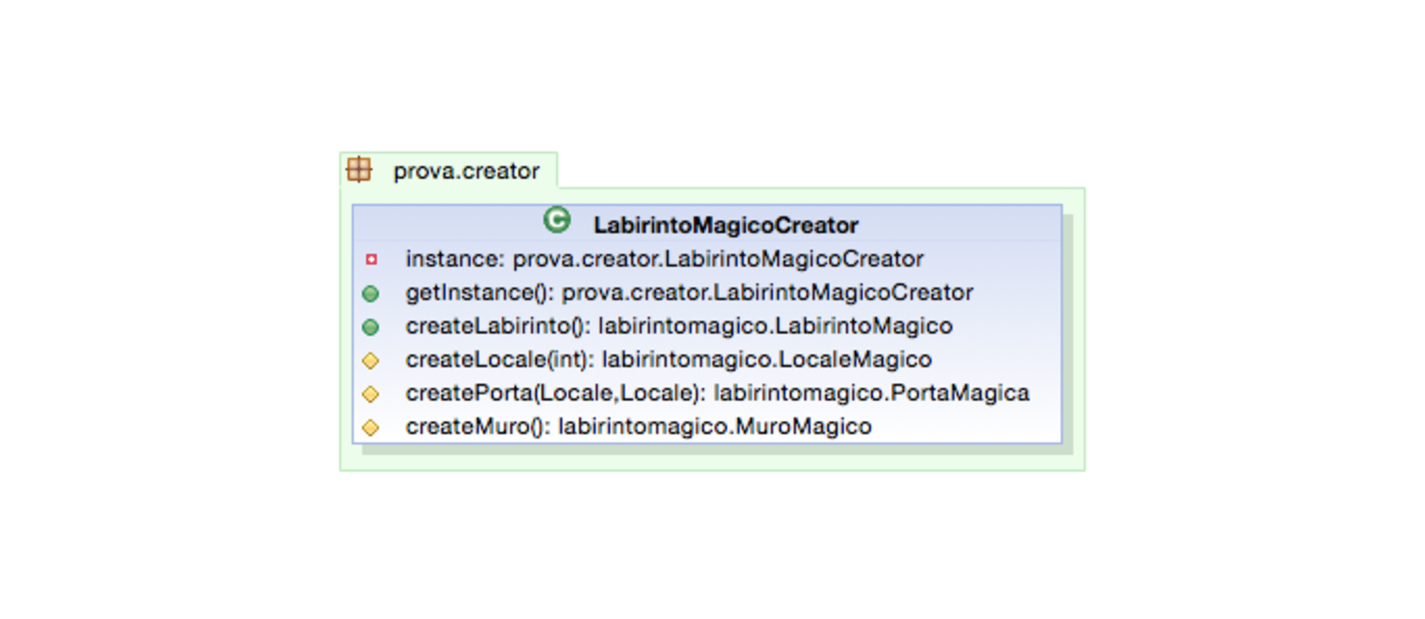
\includegraphics[width=1\textwidth]{Img/SingletonLabirintoMagico.pdf}
\caption{Class Diagram relativo alla soluzione dell'esercizio 3}
\label{Fig:labirintoMagico}
\end{figure}

\begin{lstlisting}[language=Java]
public class LabirintoMagicoCreator extends LabirintoCreator {
    private static LabirintoMagicoCreator instance=new LabirintoMagicoCreator();
	
	private LabirintoMagicoCreator(){
	}
	
	public static LabirintoMagicoCreator getInstance(){
		return instance;
	}
	
	public LabirintoMagico createLabirinto() {

		LabirintoMagico labirinto = new LabirintoMagico();
		LocaleMagico l1 = this.createLocale(1);
		Locale l2 = this.createLocale(2);

		Porta p1 = this.createPorta(l1, l2);

		labirinto.addLocale(l1);
		labirinto.addLocale(l2);

		l1.setSide(PuntoCardinale.NORD, this.createMuro());
		l1.setSide(PuntoCardinale.EST, p1);
		l1.setSide(PuntoCardinale.SUD, this.createMuro());
		l1.setSide(PuntoCardinale.OVEST, this.createMuro());

		l2.setSide(PuntoCardinale.NORD, this.createMuro());
		l2.setSide(PuntoCardinale.EST, this.createMuro());
		l2.setSide(PuntoCardinale.SUD, this.createMuro());
		l2.setSide(PuntoCardinale.OVEST, p1);

		return labirinto;
	}

	protected MuroMagico createMuro() {
		return new MuroMagico();
	}

	protected LocaleMagico createLocale(int numero) {
		return new LocaleMagico(numero);

	}

	protected PortaMagica createPorta(Locale l1, Locale l2) {
		return new PortaMagica(l1, l2);
	}
}
\end{lstlisting}


\subsection{Esercizio 4: Static Factory method}
\begin{framed}
Esercizio 4: implementare una classe che rappresenta il sacco di Babbo Natale. Il sacco di Babbo Natale non contiene elementi, ma Babbo Natale pu\`o estrarre dei giocattoli che possono essere randomicamente  Pinguini, Draghetti o un Dinosauri (con probabilit\`a 1/3 ad ogni estrazione, tranne quando gli elementi di un tipo sono finiti). Al pi\`u Babbo Natale pu\`o estrarre 20 elementi per ogni tipo. Ogni giocattolo ha un numero seriale (generato in maniera incrementale).
\end{framed}

\begin{figure}[h]
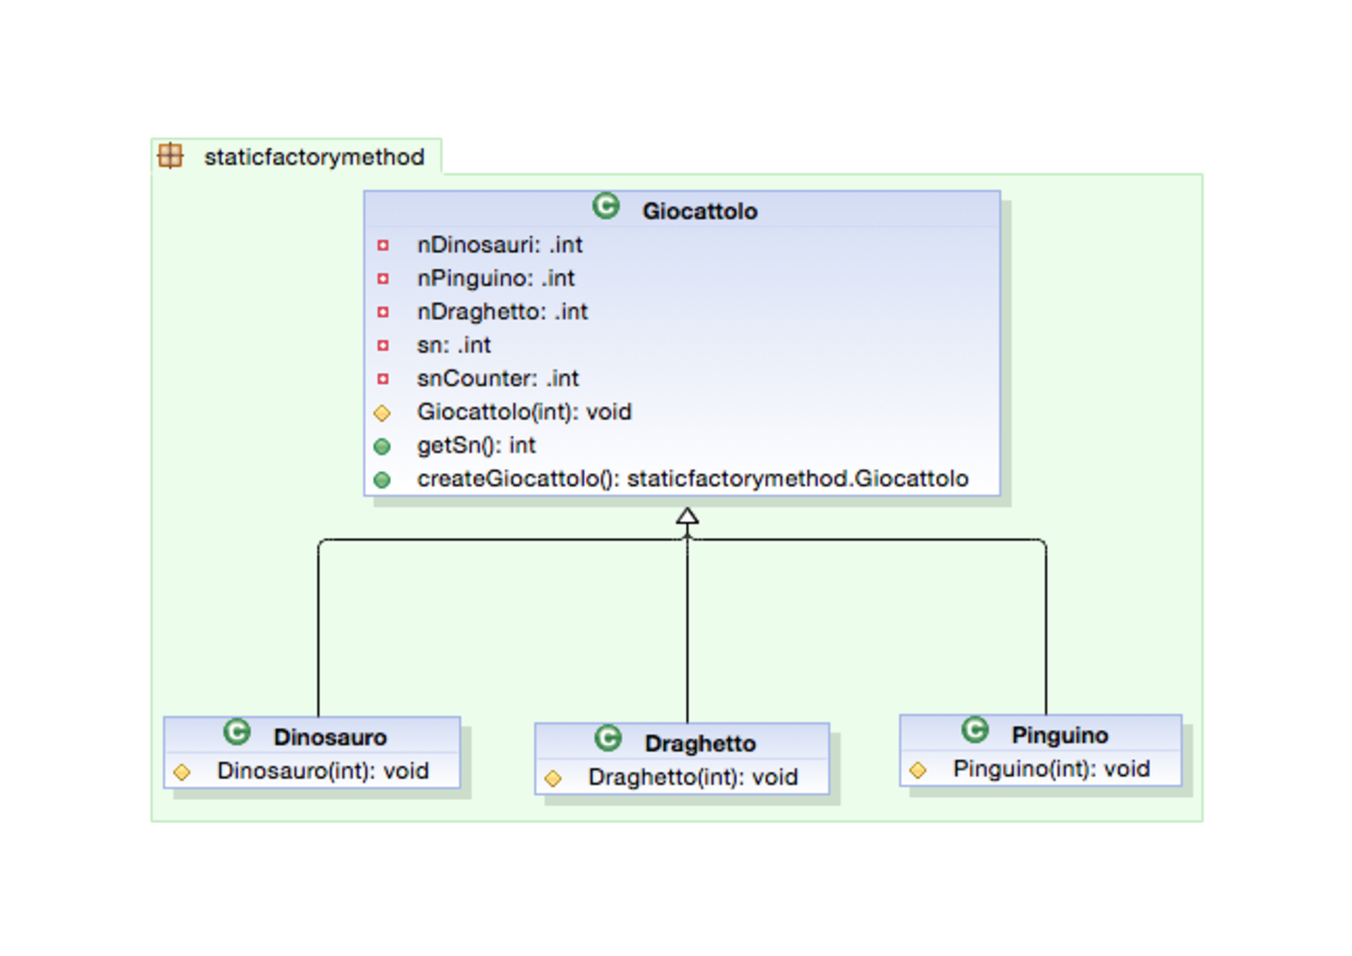
\includegraphics[width=1\textwidth]{Img/StaticFactoryMethod.pdf}
\caption{Class Diagram relativo alla soluzione dell'esercizio 4}
\label{Fig:labirinto}
\end{figure}

Decidiamo di implementare la soluzione mediante un \emph{static factory method}. Identifichiamo gli elementi in gioco: la classe \texttt{Giocattolo} e le sottoclassi \texttt{Pinguino}, \texttt{Draghetto} e \texttt{Dinosauro}. La classe giocattolo avr\`a un attibuto \texttt{sn} contenenet il serial number, pi\`u degli attributi statici \texttt{snCounter} contenente il massimo serial number assegnato fino ad ora e gli attributi statici \texttt{nDinosauri}, \texttt{nPinguini} e \texttt{nDraghetto} contenenti il numero di dinosauri, pinguini e draghetti estratti fino ad ora dal sacco di Babbo Natale.

Il metodo statico \texttt{createGiocattolo} consente di creare randomicamente un nuovo giocattolo, che pu\`o essere un \texttt{Pinguino} un \texttt{Draghetto} e un \texttt{Dinosauro} in relazione agli elementi fino ad ora estratti. Se non ci sono pi\`u giocattoli nel sacco, viene lanciata l'eccezione \texttt{GiocattoliFinitiException}.


\subsubsection{Giocattolo}
\begin{lstlisting}[language=Java]
public abstract class Giocattolo {

	private int sn;
	
	private static int nDinosauri=20;
	private static int nPinguino=20;
	private static int nDraghetto=20;
	private static int snCounter=0;

	protected Giocattolo(int sn){
		this.sn=sn;
	}

	public int getSn() {
		return sn;
	}
	
	public static Giocattolo createGiocattolo() throws GiocattoliFinitiException{
		
		if(nDinosauri==0 && nPinguino==0 && nDraghetto==0){
			throw new GiocattoliFinitiException();
		}
		List<Giocattolo> giocattoli=new ArrayList<Giocattolo>();
		if(nDinosauri>0){
			giocattoli.add(new Dinosauro(snCounter+1));
		}
		if(nPinguino>0){
			giocattoli.add(new Pinguino(snCounter+1));
		}
		if(nDraghetto>0){
			giocattoli.add(new Draghetto(snCounter+1));
		}
		Collections.shuffle(giocattoli);
		Giocattolo giocattolo=giocattoli.get(0);
		snCounter++;
		if(giocattolo instanceof Dinosauro){
			nDinosauri--;
		}
		if(giocattolo instanceof Pinguino){
			nPinguino--;
		}
		if(giocattolo instanceof Draghetto){
			nDraghetto--;
		}
		return giocattolo;
		
	}
}
\end{lstlisting}

\subsubsection{Dinosauro}
\begin{lstlisting}[language=Java]
public class Dinosauro extends Giocattolo {

	protected Dinosauro(int sn) {
		super(sn);
	}
}
\end{lstlisting}

\subsubsection{Draghetto}
\begin{lstlisting}[language=Java]
public class Draghetto extends Giocattolo {

	protected Draghetto(int sn) {
		super(sn);
	}
}
\end{lstlisting}

\subsubsection{Pinguino}
\begin{lstlisting}[language=Java]
public class Pinguino extends Giocattolo {

	protected Pinguino(int sn) {
		super(sn);
	}
}
\end{lstlisting}

\subsubsection{GiocattoliFinitiException}
\begin{lstlisting}[language=Java]
public class GiocattoliFinitiException extends Exception {

	private static final long serialVersionUID = 1L;

}
\end{lstlisting}

\section{Esercizi per casa}
\begin{itemize}
\item Esercizi:
\begin{itemize}
\item Progettare il software per la preparazione e ordinazione di pizze, installato in diverse pizzerie. Le diverse pizzerie possono creare pizze diverse a seconda di dove sono situate. Se una pizza non \`e presente nella specifica pizzeria viene lanciata una PizzaNotPresentException.
\item Fornire un’interfaccia per la creazione di famiglie di oggetti collegati. A seconda della pizzeria vengono inseriti all'interno della pizza diversi sottotipi degli ingredienti.
\item Rimuovere le  ``inutili" ripetizioni di codice presenti nella soluzione dell'esercizio 4.
\end{itemize} 
\end{itemize}

\clearpage

% ---- Bibliography ----




\addcontentsline{toc}{chapter}{Bibliography}
\bibliographystyle{alpha}
\bibliography{bib}
\nocite{*}


\end{document}

